% !TeX root = ../libro.tex
% !TeX encoding = utf8

\chapter{Ciencia de datos}\label{ch:octavo-capitulo}
\section{Introducción}
La ciencia de datos es un campo interdisciplinario que utiliza algoritmos, procedimientos y procesos para examinar grandes cantidades de datos con el fin de descubrir patrones ocultos, generar conocimientos y dirigir la toma de decisiones. Utiliza técnicas y teorías extraídas de muchos campos dentro del contexto de las matemáticas, estadísticas, programación, análisis y aprendizaje automático para descubrir conocimientos accionables a partir de conjuntos de datos.\par

En el contexto de la astrofísica, la ciencia de datos juega un papel crucial. Los astrofísicos y físicos de partículas utilizan instrumentación de última generación en telescopios y aceleradores para estudiar el Universo tanto en las escalas más grandes como en las más pequeñas. Los enormes conjuntos de datos a escala de petabytes que resultan de las diferentes observaciones y experimentos se explotan en busca de indicios, pistas que pueden arrojar luz sobre la naturaleza de la materia oscura, la energía oscura, la evolución de los agujeros negros y la física más allá del "modelo estándar" de la cosmología y la física de partículas.\par

El desafío es reformular el modelado de datos que los astrofísicos necesitan hacer de tal manera que se puedan aplicar arquitecturas de aprendizaje automático de última generación, sin comprometer el alto nivel de control de errores sistemáticos, ni la comprensión detallada de la incertidumbre estadística, que las preguntas de física que se están abordando con extrema precisión en el siglo XXI exigen. Por lo tanto, las simulaciones nos permiten probar qué teorías son consistentes con el Universo que podemos observar. Esta es una clara demostración del poder y la necesidad de la ciencia de datos para avanzar en nuestra comprensión del universo.\par


\section{Proceso de la ciencia de datos}
El proceso de ciencia de datos es un enfoque sistemático que implica varios pasos para extraer valiosos conocimientos de los datos. Comienza con la definición del problema, que implica entender los objetivos que se persiguen y formular preguntas que pueden ser respondidas con datos. Los siguientes pasos implican la recopilación y limpieza de los datos, seguidos por el análisis exploratorio de los mismos para entender los patrones y tendencias subyacentes. Esto es continuado por la construcción y evaluación del modelo para predecir resultados o descubrir estructuras dentro de los datos. Finalmente, el modelo se despliega, se contrastan los resultados con las observaciones, y los hallazgos se comunican a las partes interesadas.\par

Desde una perspectiva científica, el proceso de ciencia de datos es crucial ya que proporciona una metodología estructurada para manejar y analizar grandes volúmenes de datos. Permite a los científicos probar hipótesis, descubrir patrones, hacer predicciones e impulsar la toma de decisiones. Cada paso en el proceso sirve a un propósito específico y contribuye al objetivo general de extraer información significativa de los datos. Por ejemplo, la limpieza de datos asegura la calidad de los datos, el análisis exploratorio de datos ayuda a entender los datos, y la construcción del modelo permite hacer predicciones e inferencias.\par

Además, la naturaleza iterativa del proceso de ciencia de datos se alinea con el método científico de investigación, que implica formar hipótesis, realizar experimentos y refinar teorías basadas en los resultados. Este proceso iterativo nos permite un aprendizaje y mejora continua. Además, el énfasis en la comunicación en el proceso de ciencia de datos asegura que los hallazgos puedan ser compartidos e implementados de manera efectiva, contribuyendo al avance del conocimiento en varios campos. Por lo tanto, el proceso de ciencia de datos no sólo es un aspecto fundamental de la toma de decisiones basada en datos, sino también un contribuyente significativo al progreso científico.\par

Dentro del proceso de datos podemos enumerar una serie de etapas encaminadas a establecer una sistemática a la hora de su ejecución. El proceso no debe contemplarse como un marco rígido que no admite alteraciones al mismos, sino como que debe ser utilizado como una herramienta que debe ser adaptada a nuestras necesidades. Dependiendo de los objetivos establecidos, de la calidad de los datos que están a nuestra disposición, algunas de las siguientes etapas se harán más necesarias que otras, más intensas en lo que a la asignación de recursos se refiere. Entre los diferentes podemos enumerar los siguientes:
 
\begin{enumerate}
	\item \textit{Definición del problema} - Este es el primer paso donde definimos el problema que estás tratando de resolver. Implica entender los objetivos de la investigación, para a continuación formular preguntas que pueden ser respondidas con datos e identificar las fuentes de datos necesarias.
	\item \textit{Recopilación de datos} - En este paso, recopilamos los datos necesarios para nuestro análisis. Esto podría implicar la consulta de sitios web, el acceso a bases de datos, generación de simulaciones.
	\item \textit{Limpieza de datos} - Una vez que tenemos los datos recopilados, es hora de limpiarlos. Esto implica manejar valores faltantes, eliminar duplicados, corregir errores y lidiar con valores atípicos.
	\item \textit{Análisis exploratorio de datos} - Este es un paso crucial donde exploramos y visualizamos los datos para entender los patrones subyacentes, las tendencias y los valores atípicos. Es una paso fundamental porque nos ayuda a generar conocimiento y formar hipótesis para un análisis más profundo.
	\item \textit{Ingeniería de características} - Esto implica crear nuevas características a partir de las existentes para representar mejor los patrones subyacentes en los datos. Es un paso esencial para mejorar el rendimiento de los modelos de aprendizaje automático. 
	\item \textit{Construcción del modelo} - Aquí, elegimos un modelo apropiado, lo entrenamos con los datos que previamente hemos obtenido para luego evaluar su rendimiento. Normalmente esto implica dividir los datos en conjuntos de entrenamiento y prueba, seleccionar un algoritmo correcto y fijar sus parámetros.
	\item \textit{Evaluación del modelo} - En este paso, evaluamos el rendimiento del utilizando métricas apropiadas. Es importante usar una métrica que se alinee con los objetivos que hemos prefijados en el paso inicial.
	\item \textit{Despliegue del modelo} - Una vez que estamos satisfecho con el rendimiento del modelo, es hora de desplegarlo. Esto podría implicar integrar el modelo en un sistema de producción, establecer un sistema de monitoreo y desarrollar un plan para el mantenimiento del mismo.
	\item \textit{Comunicación} - Finalmente, comunicamos nuestros hallazgos a las partes interesadas. Esto podría implicar la creación de artículos científicos, informes, o presentaciones que expliquen claramente tu metodología, hallazgos e implicaciones de negocio de nuestro trabajo.
\end{enumerate}

Como hemos adelantado, los pasos anteriores no de dejan de ser un marco de trabajo genérico que debe de ser adaptado a nuestras necesidades específicas. En nuestro caso en particular, no hemos recurrido al uso de herramientas de aprendizaje automático, por lo que la correspondiente etapa no ha formado parte de nuestro proceso de ciencia de datos. Del mismo modo, nuestro modelo no ha sido incorporado, integrado con ningún sistema. De momento este no ha sido el caso pero no sería descabellado pensar que pudiese pasar a incorporarse como una extensión a la herramienta que hemos utilizado para nuestras simulaciones, si lo autores de la misma lo considerasen oportuno.


\section{Catálogos de datos}
En la vastedad del cosmos, los catálogos de datos se alzan como pilares fundamentales para los investigadores en astrofísica. Estos catálogos, que contienen descripciones detalladas y metadatos, permiten comprender y acceder a la riqueza de información cósmica. Proporcionan contexto esencial para comprender los datos recopilados por telescopios y observatorios, permitiendo a los científicos explorar las coordenadas celestiales, las magnitudes estelares y las características espectrales.\par

Sus propiedades fundamentales son múltiples: en primer lugar, los catálogos permiten una búsqueda eficiente. En un campo donde la cantidad de datos es abrumadora, esta eficiencia es vital. Además, fomentan la colaboración científica al proporcionar un acceso centralizado. Los metadatos, que describen y resumen la entradas de los catálogos, son la clave para evaluar la calidad y actualidad de los datos.\par

Los catálogos proporcionan una base de referencia para comparar las propiedades simuladas con las observaciones reales. Además, nos permiten calibrar los parámetros de los modelos y refinarlos mediante la comparación detallada entre las características de las estrellas simuladas y las observadas.\par


\subsection{Gaia}
El catálogo Gaia \citep{Mignard2005} es un mapa tridimensional completo de la Vía Láctea, creado utilizando datos del telescopio espacial Gaia. Éste contiene datos de alrededor de 1.46 millardos de estrellas, entre los que se encuentra sus posiciones en el cielo, paralaje y movimiento propio. Además, incluye sus magnitudes en diferentes bandas espectrales para una gran cantidad de ellas. El catálogo Gaia es particularmente útil para estudiar estrellas similares al Sol, ya que proporciona un censo único de estrellas dentro de 100 pc de nuestro Sol. Esto lo convierte en un recurso invaluable para los astrónomos y astrofísicos que buscan comprender mejor las propiedades y la evolución de estas estrellas.\par

\subsection{Gaia-ESO Spectroscopic Survey - (GES)}
El estudio Gaia-ESO (Gaia-ESO Survey, GES) \citep{Gilmore2012,Randich2013,Randich2022} es un catálogo público enfocado al análisis espectroscópico de un número importante de estrellas recogidas en el catálogo Gaia. Se llevó a cabo con el instrumento espectrógrafo multielemento de fibra de gran conjunto (Fibre Large Array Multi Element Spectrograph, FLAMES) y el espectrógrafo Echelle ultravioleta y visual (Ultraviolet and Visual Echelle Spectrograph, UVES) en el VLT. Su objetivo es proporcionar una visión homogénea de las distribuciones de cinemática y abundancias elementales en la Vía Láctea, en el campo y en cúmulos abiertos (Open Cluster, OC), hasta magnitud 19.\par 

Dentro de la iniciativa GES se han observado más de 110 000 estrellas, proporcionando velocidades radiales y rotacionales proyectadas, parámetros estelares tales como: temperatura efectiva, gravedad superficial y metalicidad, abundancias de varios elementos, entre los que se encuentra el litio, para aproximadamente 1/3 de la muestra, y parámetros específicos para rastrear la acreción y actividad en estrellas jóvenes. El catálogo GES es único en lo que se refiere a la observación de estrellas de todos los tipos espectrales con análisis dedicados y especializados, lo que la hace particularmente útil para estudiar estrellas similares al Sol.\par


\section{Herramientas}
\subsection{Modules for Experiments in Stellar Astrophysics - MESA}
Para la realización de este tesis doctoral nos hemos apoyado en la herramienta de evolución estelar MESA (Modules for Experiments in Stellar Astrophysics). MESA ha jugado un papel fundamental en nuestra investigación y por ello, debido a su importancia, le hemos dedicado un capítulo en exclusiva en el que entramos a fondo en sus características, estructura, módulos que lo componen, y muy especialmente en cómo extender la física que incorpora sus modelos mediante la programación de nuestras propias rutinas.\par


\subsection{Octave} \label{sec:tool_octave}
GNU Octave es un lenguaje de programación de alto nivel destinado principalmente a cálculos numéricos. Es un conjunto de software libre y de código abierto que proporciona una interfaz de línea de comandos conveniente para resolver problemas lineales y no lineales numéricamente. La sintaxis de Octave es en gran medida compatible con MATLAB, lo que lo convierte en una alternativa popular para los usuarios que necesitan una solución rentable.\par 

Esta herramienta también proporciona amplias capacidades gráficas para la visualización y manipulación de datos. Octave puede ser extendido por paquetes, permitiendo a los usuarios añadir más funcionalidades según sea necesario. Puede ser ejecutado en modo visual, como una consola, o invocado como parte de un script de entorno. Octave está disponible para varios sistemas operativos, incluyendo GNU/Linux, macOS, BSD y Microsoft Windows.

\subsection{Tool for OPerations on Catalogues And Tables - TOPCAT} \label{sec:tool_topcat}
TOPCAT, acrónimo de \textit{Tool for OPerations on Catalogues And Tables}, es un visor y editor gráfico altamente versátil e interactivo para datos tabulares. Está diseñado para trabajar con datos astronómicos, pero puede ser utilizado para cualquier tipo de datos en formato tabular. Proporciona un entorno dinámico donde los datos pueden ser cargados, visualizados, editados y analizados. TOPCAT soporta varios formatos de datos y puede gestionar tanto archivos locales como remotos, lo que lo convierte en una herramienta flexible para la manipulación de datos.\par

En cuanto a la extracción de datos, TOPCAT permite a los usuarios ver y editar datos de celdas a través de un navegador, y tiene visores para imágenes y espectros. También se incluye un visor de trazado del cielo para datos astronómicos. Además, proporciona funciones estadísticas para analizar los datos, y capacidades de coincidencia cruzada para comparar diferentes catálogos. La herramienta también soporta scripting para tareas automatizadas. Estas características hacen de TOPCAT una herramienta integral para la extracción y análisis de datos en el campo de la astronomía y más allá.\par

TOPCAT es particularmente útil para el observatorio virtual (Virtual Observatory, VO). Ésta es una aplicación de escritorio para el análisis interactivo de datos en formato tabular, especialmente catálogos de fuentes. TOPCAT puede acceder a servicios de datos externos. También puede comunicarse con otras herramientas astronómicas a través del protocolo simple de mensajería de aplicaciones (Simple Application Messaging Protocol, SAMP). Esto permite una integración perfecta de TOPCAT en el entorno del VO, permitiendo a los usuarios recuperar y analizar datos de varios servicios.\par

Cuando se trata de extraer datos de diferentes catálogos astronómicos, TOPCAT proporciona una gama de funcionalidades, como las de leer y escribir tablas en varios formatos como FITS, VOTable, CSV. Esto hace posible trabajar con una amplia variedad de catálogos astronómicos. Por ejemplo, se puede usar TOPCAT para acceder a un catálogo de estrellas contenidas en la base de datos Gaia. Además, TOPCAT ofrece características para el cruce de correspondencias, que es crucial al comparar diferentes catálogos. En el Listado \ref{lst:consulta} podemos observar la consulta que hemos utilizado para seleccionar del catálogo GES las estrellas pertenecientes a OC's con un nivel de confianza >= 95\%. Para cada una de ellas obtenemos su temperatura efectiva, la gravedad superficial, su metalicidad, la abundancia de Li, y los valores de error asociados a cada uno de esos parámetros.\par


\begin{lstlisting}[language=SQL, float, caption={Consulta TOPCAT sobre el catálogo GES DR5 para obtener los componentes de los cúmulos abiertos para los cuales se ha determinado una pertenecia mínima del 0.95\%. Las columnas obtenidas informan sobre la identificador de la estrella, $\teff$, $\gsurf$, $\feh$, A(Li) y sus errores asociados, y el identificador del cúmulo al que pertenece.}, label={lst:consulta}]
	SELECT object,teff,e_teff,logg,e_logg,feh,e_feh,li1,e_li1,ges_fld
	FROM ges_dr5 
	WHERE ges_fld IN (
	SELECT DISTINCT ges_fld
	FROM ges_dr5 
	WHERE ges_type 
	LIKE 'GE_CL%' 
	OR ges_type LIKE 'GE_SD_OC%' 
	OR ges_type LIKE 'AR_CL%' 
	OR ges_type LIKE 'AR_SD_OC' )
	AND mem3d >= 0.95
	AND li1 IS NOT NULL
	AND feh IS NOT NULL
	AND ges_fld IS NOT NULL
	AND teff IS NOT NULL
	AND logg IS NOT NULL
	AND nn_teff IS NOT NULL
	AND nn_logg IS NOT NULL
	AND nn_feh IS NOT NULL
	ORDER BY ges_fld
\end{lstlisting}

Antes de poder realizar la consulta hay que localizar el catálogo sobre el que ejecutar la búsqueda. Como acabamos de comentar, TOPCAT es una herramienta polivalente y que sobresale a la hora de acceder a diferentes fuentes datos. Mediante el protocolo de acceso a tablas (Table Access Protocol, TAP) TOPCAT ofrece la posibilidad de realizar búsquedas entre los catálogos que soportan TAP mediante el uso de palabras claves o propiedades de los catálogos. En la Figura \ref{fig:tap_ges_service} vemos el resultado ofrecido tras realizar una búsqueda en los catálogos disponibles que están relacionados con GES.\par

\begin{figure}
	\centering
	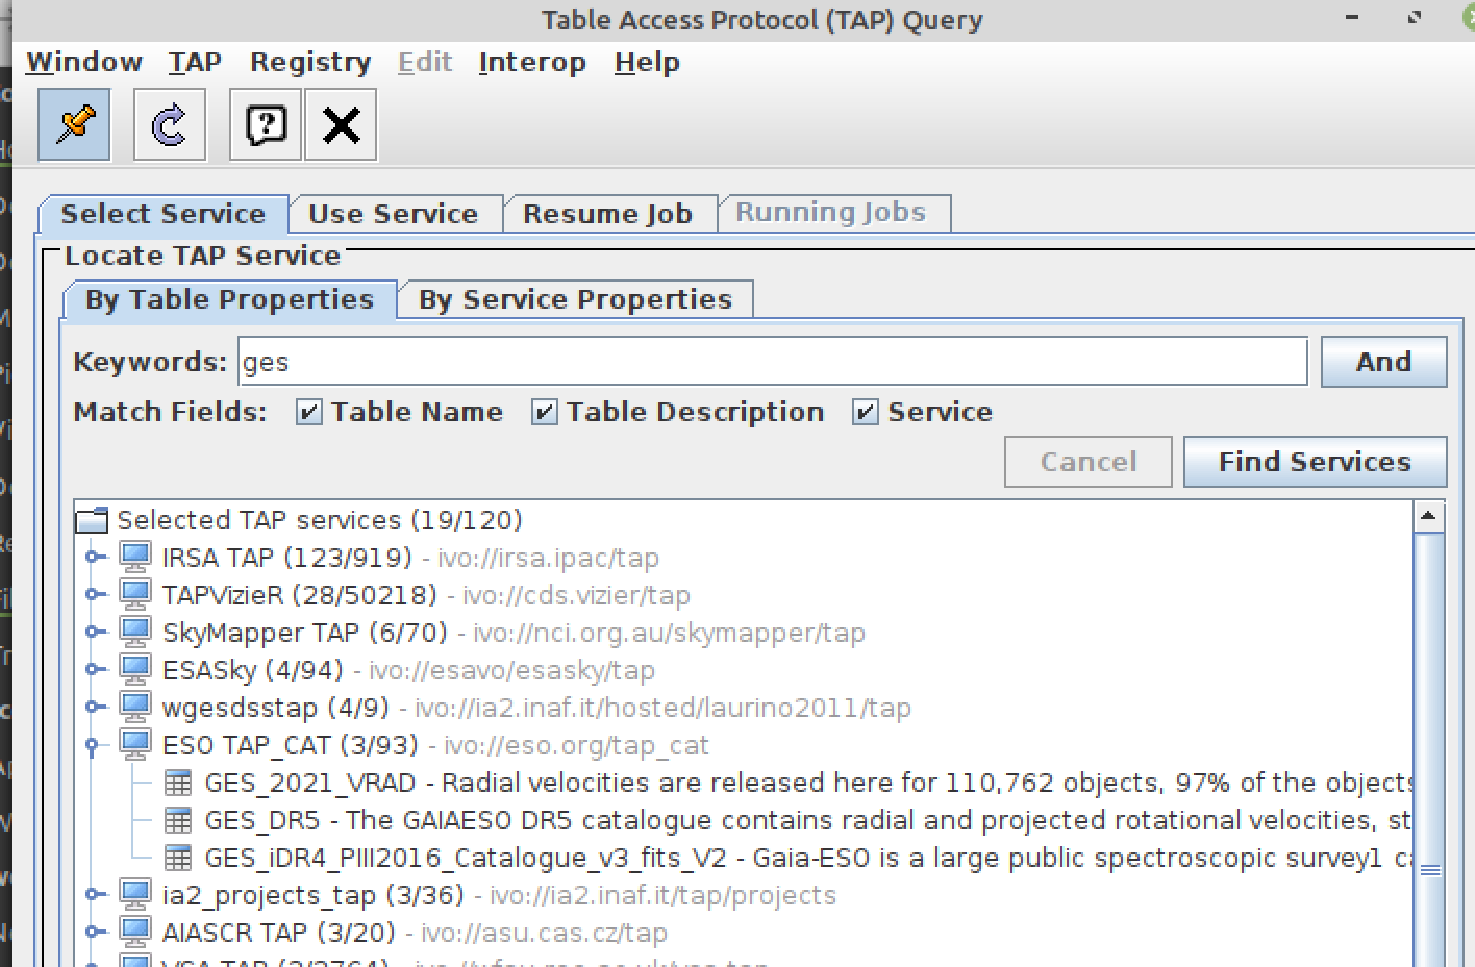
\includegraphics[width=0.7\textwidth]{img/tesis/tap_ges_service.pdf}
	\caption{Búsqueda de catálogos con información de GES. Mediante el uso de TAP, TOPCAT es capaz de ofrecer una lista de catálogos que poseen información referente a GES. En nuestro caso, hemos seleccionado el catálogo publicado por la ESO.}
	\label{fig:tap_ges_service}
\end{figure}


Un ejemplo similar, pero esta vez orientado a localizar catálogos con información de cúmulos abiertos es el que nos ofrece la Figura \ref{fig:tap_query_oc}. Una vez seleccionado el catálogo, TOPCAT nos ofrece la posibilidad de obtener detalles adicionales sobre los esquemas y tablas que los conforman. Esta información es muy útil a la hora de realizar nuestras consultas, ya que de ella podemos extraer no solo las columnas incluidas en la diferentes tablas, sino también el tipo de información que contiene (necesario cuando el nombre de la columna no es suficientemente explicativo), tipo de datos (numérico, texto, fecha...), columnas claves, referencia entre tablas (claves foráneas), y más información relevante. Este conjunto de información adicional es lo que se conoce como meta-información o meta-datos asociados a la tabla (ver Figura \ref{fig:tap_table_metadata}).\par


\begin{figure}
	\centering
	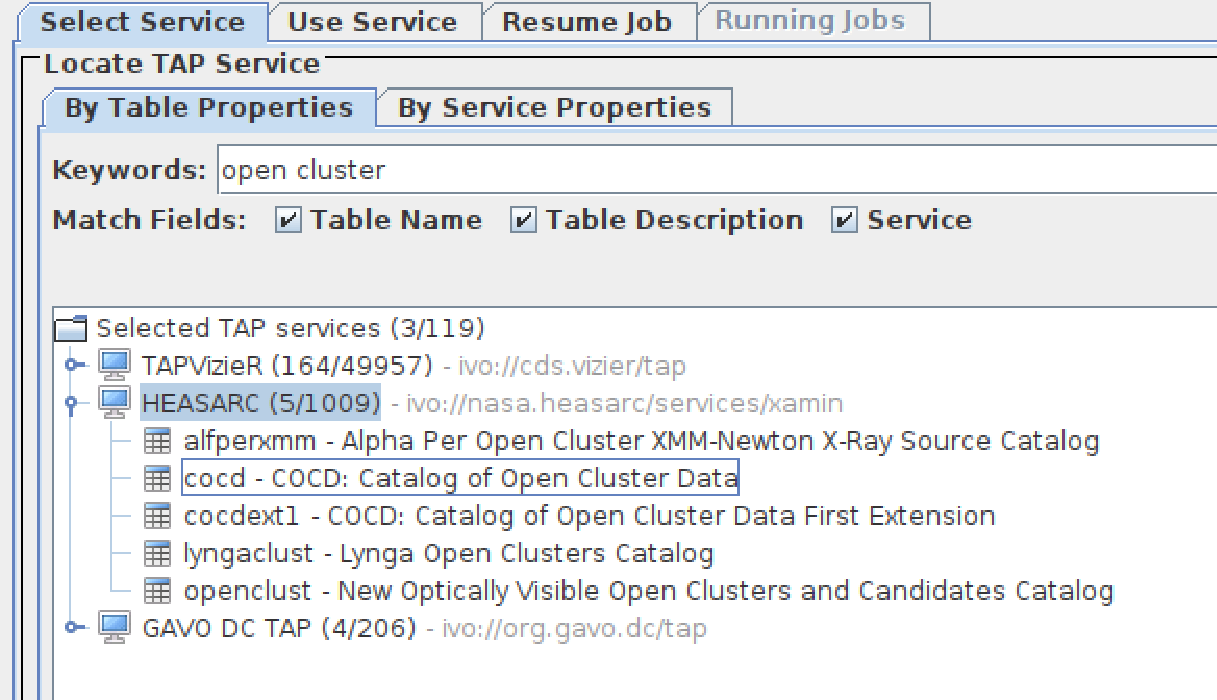
\includegraphics[width=0.7\textwidth]{img/tesis/tap_service.pdf}
	\caption{Búsqueda de catálogos con información relacionada con cúmulos abiertos.}
	\label{fig:tap_query_oc}
\end{figure}

\begin{figure}
	\centering
	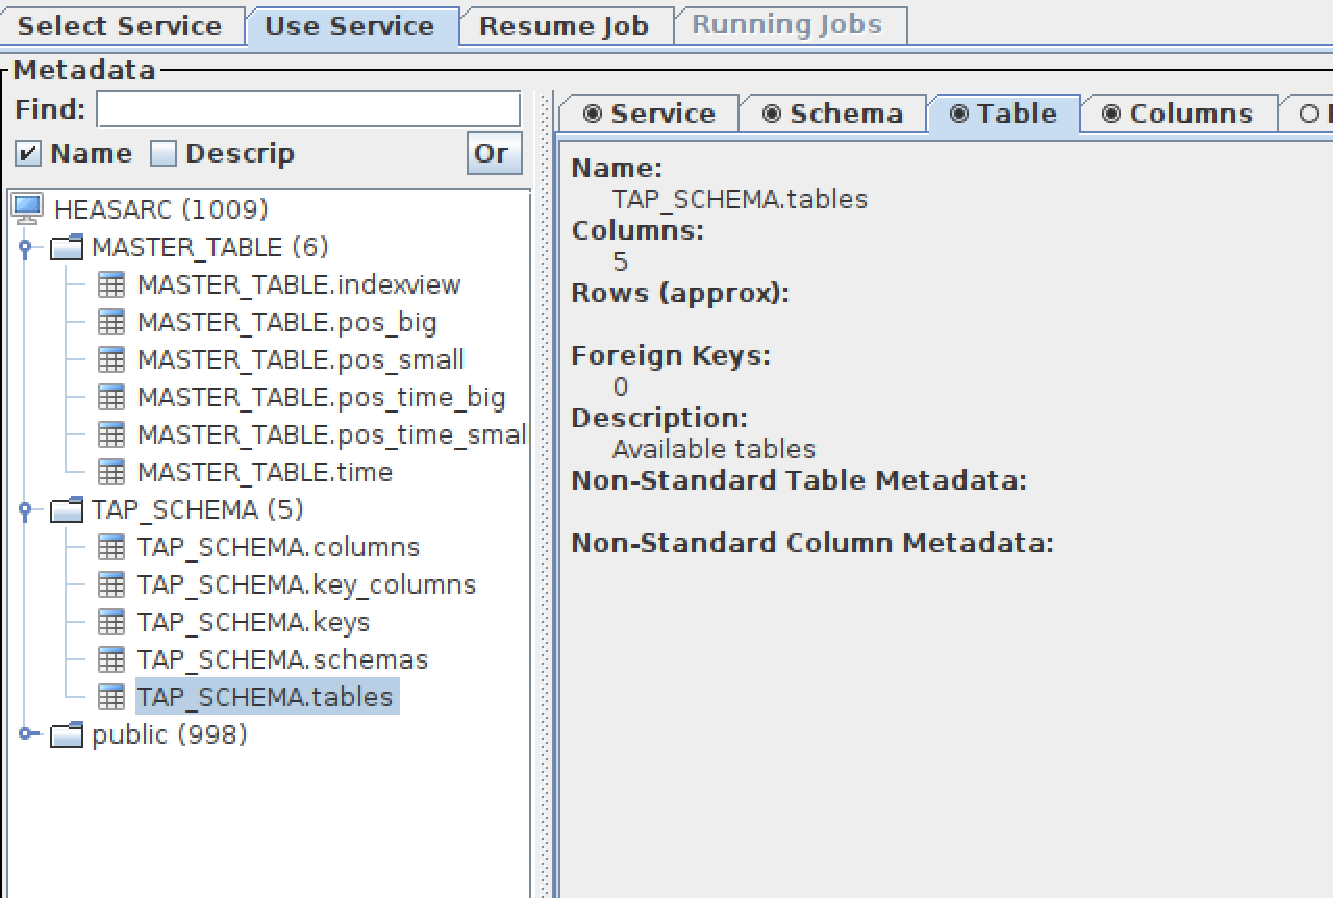
\includegraphics[width=0.7\textwidth]{img/tesis/tap_schema.pdf}
	\caption{Vista con meta-información asociada a una tabla.}
	\label{fig:tap_table_metadata}
\end{figure}

TOPCAT también es capaz de mostrar las diferentes tablas contenidas dentro de un esquema. Un esquema define cómo se organizan los datos dentro, las tablas que los contienen. Esto incluye restricciones lógicas, como nombres de tablas, campos, tipos de datos y las relaciones existente entre ellas (ver Figura \ref{fig:tap_schema_detail}).\par

\begin{figure}
	\centering
	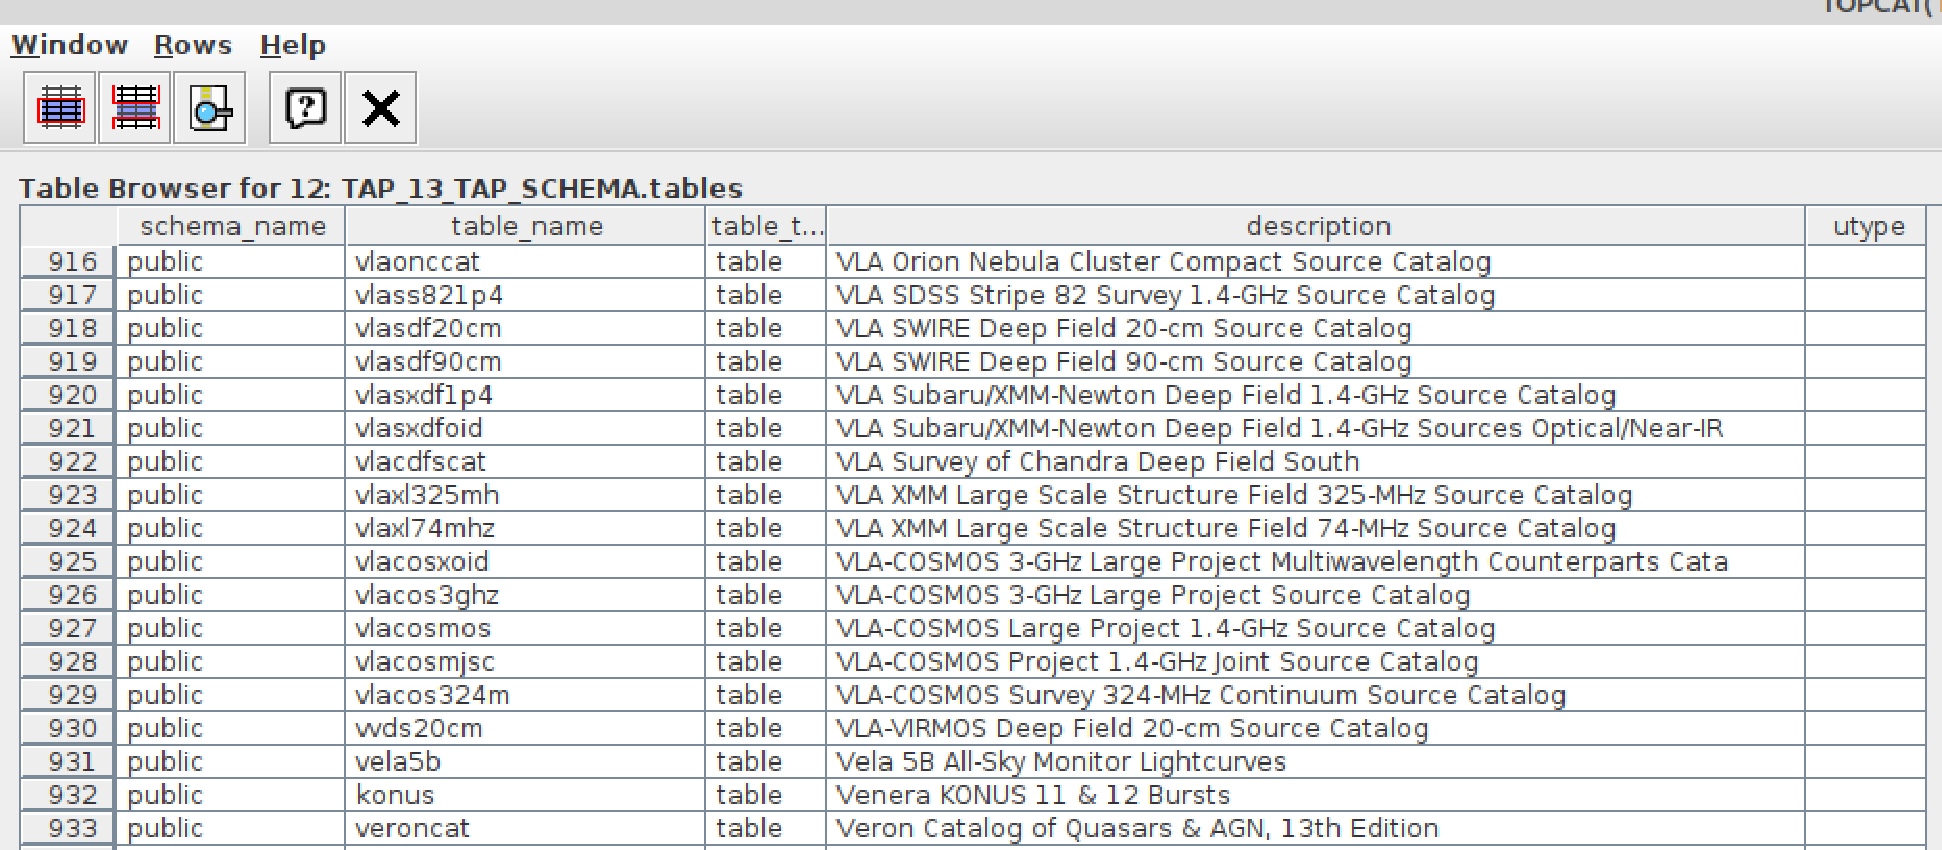
\includegraphics[width=0.7\textwidth]{img/tesis/tap_schema_detail.pdf}
	\caption{Vista con lista de tablas contenida en un esquema.}
	\label{fig:tap_schema_detail}
\end{figure}


\section{Selección de datos}
\subsection{El binomio Gaia-GES}
La combinación de los datos de los catálogos Gaia y GES puede proporcionar una visión completa de las propiedades y evolución de las estrellas similares al Sol. El catálogo Gaia proporciona datos de posición precisos y paralajes, mientras que la GES ofrece información espectroscópica detallada. Esta combinación permite una comprensión más completa de estas estrellas, incluyendo su cinemática, composiciones químicas y potencial para albergar planetas. Al proporcionar una perspectiva más amplia y detallada de estas estrellas, podemos obtener una comprensión más profunda de las propiedades y evolución de las estrellas similares al Sol, lo que representa una fuente de información que se antoja invaluable para la investigación en astrofísica. Estamos ante un conjunto de herramientas poderoso para cualquier astrofísico que estudie estrellas similares al Sol.\par

En el caso de las abundancias de litio, y como ya hemos apuntado, éste es un elemento clave en el estudio de la astrofísica estelar, ya que su abundancia puede proporcionar información valiosa sobre la edad y la historia de las estrellas. Sin embargo, la determinación precisa de las abundancias de litio puede ser un desafío debido a la complejidad de las líneas espectrales de este elemento. GES nos asiste en nuestra investigación aportando su análisis especializado y dedicado de estrellas de todos los tipos espectrales, convirtiéndose así en una herramienta fundamental a la hora de afrontar este desafío.\par

Por otra parte, tenemos información precisa sobre la velocidad angular de las estrellas. Gaia es capaz de medir la velocidad angular de las mismas con una precisión sin precedentes, y ésta nos aporta información crucial para estudiar y entender su rotación, evolución y estructura interna. Combinado esta información con las abundancias de litio podemos establecer hipótesis y validar las mismas acerca del impacto de la velocidad angular sobre este elemento. Paralelamente, la velocidad angular juega un papel crucial en el análisis de la presencia e intensidad de un campo magnético en las estrellas. Los campos magnéticos son responsables de la pérdida de momento angular en las estrellas jóvenes y son la principal fuente de energía detrás de una amplia gama de fenómenos dinámicos (llamaradas, emisión de rayos X, manchas estelares) que ocurren en las capas superficiales del Sol y otras estrellas. Por lo tanto, la medición precisa de la velocidad angular de una estrella puede proporcionar información valiosa sobre la presencia e intensidad de su campo magnético.\par

Otra fuente de información valiosa para nuestra investigación procedente de ambos catálogos es la referida a los cúmulos abiertos. Los cúmulos abiertos son grupos de estrellas que se formaron a partir de la misma nube de gas y polvo. Por lo tanto, todas las estrellas de un cúmulo abierto tienen aproximadamente la misma edad y composición química inicial. Esto los convierte en laboratorios naturales para estudiar la evolución de las estrellas a través de sus diferentes etapas. Gaia ha observado una gran cantidad de cúmulos abiertos, proporcionando datos detallados sobre sus miembros. En paralelo, GES también ha observado un gran número de ellos en un rango amplio de edades. La combinación de ambas fuentes permite estudiar la estructura y dinámica de este tipo de cúmulos, y usarlos para restringir y mejorar los modelos de evolución estelar, algo que hemos puesto en práctica en nuestra investigación.\par

Como acabamos de adelantar, la investigación de los campos magnéticos en estrellas similares al Sol, y en particular de aquéllas que se encuentran en cúmulos abiertos, se beneficia enormemente de los datos proporcionados por ambos catálogos. Los campos magnéticos juegan un papel importante en todas las etapas de la evolución estelar. En estrellas similares al Sol se generan en las capas convectivas exteriores. Estudiar los campos magnéticos a gran escala de estas estrellas puede mejorar nuestra comprensión sobre los mismos y proporcionar restricciones observacionales para los modelos que estudian cómo se generan, la topología que presentan y sus intensidades. Los datos de los catálogos nos asisten a la hora de identificar y estudiar las estrellas con alta actividad magnética, lo que puede proporcionar pistas sobre la dinámica interna de las mismas y su evolución. Combinando esta información con la velocidad angular, nos puede proporcionar indicios de cómo se interrelacionan ambos fenómenos. Adicionalmente, cruzando estos datos con la información de los cúmulos abiertos, obtenemos una visión más clara de cómo los campos magnéticos varían entre las estrellas de la misma edad y composición química.\par


\subsection{Selección de parámetros}
Como indica su nombre, GES pretende complementar los datos sobre paralajes y movimientos propios del satélite Gaia con información extremadamente precisa sobre velocidades radiales (Radial Velocity, RV), litio y química en general. La primera publicación de datos de Gaia (GDR1) \citep{Brown2016} data de 2016 y contiene información sobre los primeros 14 meses funcionamiento de la misión. La segunda publicación de datos de Gaia (GDR2) \citep{Brown2018} publicada en 2018, contiene posiciones, paralajes y movimientos propios de unos 1 300 millones de fuentes, junto con información fotométrica. La tercera publicación de datos de Gaia, la Gaia Early Data Release 3 (GEDR3) \citep{Brown2021} y la Gaia Data Release 3 (GDR3) \citep{Brown2022}, aportan medidas actualizadas y más precisas. GES las mejora y en su última versión (DR5.0) incluye todos los parámetros astrofísicos derivados por el consorcio Gaia-ESO \citep{Gilmore2022}. De interés para nuestra línea de investigación son:
\begin{itemize}
	\item Velocidades radiales y proyectadas
	\item Parámetros estelares (temperatura efectiva, gravedad superficial y metalicidad)
	\item Abundancias de varios elementos, entre ellos el litio
	\item Parámetros específicos para rastrear la acreción y la actividad en estrellas jóvenes
	\item Probabilidad de pertenencia a cúmulos
\end{itemize}


\subsection{Selección de cúmulos abiertos}
GES DR5.0 proporciona información sobre 114 324 estrellas véase \citep[véase][para más detalles]{Gilmore2022}. Para nuestra investigación estamos interesados en considerar aquéllas que pertenecen a OCs, para ello seleccionamos aquellos registros GES que cumplen alguna de las siguientes condiciones:

\begin{itemize}
	\item GE\_CL: observado por GES, campo del programa OC
	\item GE\_SD\_OC: observado por GES, campo estándar OC
	\item AR\_CL: Observación del Archivo ESO, campo de programa OC
	\item AR\_SD\_OC: Observación de archivo, campo estándar OC
\end{itemize}
	
Como resultado de este primer filtrado, el número de registros seleccionados se reduce a 43 299. Sobre este subconjunto de datos realizamos otro filtrado, esta vez dirigido a seleccionar aquellos que ofrecen información no nula sobre los siguientes atributos:

\begin{itemize}
	\item Metalicidad
	\item Abundancia de litio
	\item Identificador de campo GES
	\item Temperatura efectiva
	\item Gravedad superficial
	\item Probabilidad de pertenencia a un cúmulo (>= 0.95\%)
\end{itemize}

Este segundo filtrado reduce la población de estrellas a considerar a un total de 5 895 registros que se distribuyen entre los 64 OCs listados en la Tabla \ref{tab:oc_full_list}.\par

Como datos de referencia tomamos un subconjunto de las observaciones obtenidas por GES. Este subconjunto consiste en aquellas estrellas que pertenecen a OCs, y entre ellas se encuentran potenciales gemelas "ocultas" de nuestro Sol. Para identificar estas últimas, procedemos a realizar una selección adicional, esta vez utilizando los valores dados por nuestros modelos durante las simulaciones para la metalicidad ($\feh$), la temperatura efectiva ($\teff$) y la gravedad superficial ($\gsurf$). Por último, nos quedan las estrellas para las que las observaciones de GES han medido valores congruentes con los resultados de nuestros modelos, a partir de los cuales obtenemos finalmente sus abundancias de litio.\par

\subsection{Selección de gemelos solares} \label{sec:gemelos_solares}
Una vez preseleccionadas las estrellas pertenecientes a los OCs, el interés se centra en identificar las más parecidas a nuestro Sol, es decir, las gemelas solares. Esto nos lleva a preguntarnos qué parámetros estelares debemos tener en cuenta para clasificar una estrella como gemela solar. Encontrarlos nos ayudaría a averiguar el origen de nuestro Sol y a obtener información sobre las condiciones que prevalecían en los OC en los que nacieron.\par

Ya se han realizado varios intentos de encontrar hermanos y gemelos solares. Los primeros se refieren a estrellas que se formaron en el mismo cúmulo que el Sol y, por tanto, deberían tener edades y abundancias químicas muy similares a las de éste \citep[ver][y referencias en él]{Adibekyan2018}. Por otro lado, según \cite{Strobel1996}, se consideran gemelos solares a aquellas estrellas que poseen parámetros físicos fundamentales como $\teff$, $\gsurf$, $\feh$, propiedades fotométricas, composición química, edad, luminosidad, rotación y campos magnéticos similares, si no idénticos, a los del Sol. Localizar estos gemelos solares supone un reto formidable debido a los estrictos criterios y a su dispersión por toda la Vía Láctea.\par 

No es de extrañar que los métodos de búsqueda aplicados se orienten a encontrar las candidatas basándose en sus propiedades cinemáticas. Luego se comparan sus temperaturas, metalicidades y abundancias químicas con las de nuestro Sol. En nuestro estudio, ampliamos los criterios de selección añadiendo la gravedad superficial y la edad de la estrella. Estos dos nuevos parámetros representan un ajuste fino del proceso de búsqueda de candidatos a gemelos. Los catálogos Gaia y GES no proporcionan la edad estimada de los OCs, así que necesitamos recurrir a los resultados obtenidos en el trabajo de \cite{Bragaglia2022} (ver Figura \ref{fig:open_cluster_sample}). Utilizamos la edad de los OCs indicada en la tabla \ref{tab:oc_reduced_list} y los datos obtenidos a partir del conjunto de simulaciones MESA iniciadas con diferentes $\omegaini$, donde $\omegaini = \oomegac$, $\Omega$ es la velocidad angular de la estrella en la superficie estelar, y $\omegac$ es la velocidad superficial en el ecuador de una estrella en rotación donde la fuerza centrífuga equilibra la gravedad newtoniana. La edad derivada de estas simulaciones proporciona un parámetro clave para nuestro análisis. Esta información nos permite determinar los demás parámetros de simulación, que posteriormente utilizaremos para compararlos con los valores asociados a las estrellas pertenecientes a los OCs preseleccionados.\par

\begin{table}
	\centering
	\begin{tabular}{ll} 
		\hline
		Parámetro estelar & Intervalo de selección\\
		\hline
		Edad OC & $\pm0.1\%$ \, para edad < 1 Ga \\
		& $\pm0.15\%$ \, para edad $\geq$ 1 Ga \\
		$\teff$ & $\pm 50.0 \, \Kelvin$ \\
		$\gsurf$ & $\pm 0.05 \, \dex$\\
		$\feh$ & $\pm 0.05 \, \dex$\\
		\hline
	\end{tabular}
	\caption{Parámetros e intervalos de selección aplicados durante el proceso de triaje sobre los componentes del OC.}
	\label{tab:sel_params}
\end{table}

De las aproximadamente 5 900 estrellas identificadas, seleccionamos aquellas cuyos valores de $\feh$, $\teff$ y $\gsurf$ se encuentran en los intervalos correspondientes definidos en la Tabla \ref{tab:sel_params} y según el siguiente proceso de filtrado: a partir de los valores dados por nuestras simulaciones para los parámetros listados en la Tabla \ref{tab:sel_params}, procedemos a seleccionar de los distintos OCs aquellas estrellas que tienen valores dentro de los intervalos establecidos. En concreto, para la edad estimada de un determinado cúmulo, establecemos un intervalo de $\pm$0.1 para OCs jóvenes (edad < 1 Ga) y $\pm$0.15 para contrapartes más viejas (edad >= 1 Ga) \citep{Cantat-Gaudin2020}[véase][para más detalle sobre los valores referidos]. Este intervalo dependiente de la edad sirve como base para seleccionar los pasos de tiempo de simulación que se alinean con los límites de edad inferior y superior de cada grupo. Una vez encontrados estos dos pasos temporales, se reúnen los valores límite asociados para $\teff$, $\gsurf$ y $\feh$. Con estos rangos de valores procedemos entonces a seleccionar en cada uno de los OCs aquellas estrellas que tienen valores para estos mismos parámetros dentro de ellos. De esta forma obtenemos finalmente las estrellas candidatas a ser comparadas con los resultados de la simulación.\par

El resultado del proceso de filtrado puede observarse en las siguientes tablas. En la Tabla \ref{tab:oc_reduced_list} se agrupan los OCs que han aportado alguno de sus miembros en las simulaciones que hemos realizado. Para un determinado OC se informa del número de estrellas que se han seleccionado en las diferentes simulaciones. Por otra parte, las tablas \ref{tab:oc_m67} y \ref{tab:oc_ngc2516} resumen el subconjunto de componentes de los OCs M67 y NGC2516 seleccionados durante las simulaciones para modelos inicializados con $\omegaini = 0.14$. Cada una de las tablas enumera el identificador GES de la estrella y los rangos de $\teff$, $\gsurf$, $\feh$, A(Li), el error estimado de la A(Li) y edad estimada utilizados en la simulación. Estos valores representan los rangos de valores en los que se ha basado el filtrado.


\newpage
\KOMAoptions{paper=landscape,pagesize}
\recalctypearea

\begin{longtable}[c]{|l l l l || c c c c c c c c c c|}
	\hline
	& & & & & & & & $\omegaini$ & & & & & \\
	Cúmulo Abierto & Edad(Ga) & [Fe/H] & $N_*$ & 0.095 & 0.10 & 0.105 & 0.11 & 0.115 & 0.12 & 0.125 & 0.13 & 0.14 & 0.1425\\
	\hline
	Berkeley 21 & 2.138 & -0.21 & 744 & 0 & 0 & 0 & 0 & 0 & 1 & 1 & 1 & 1 & 1\\
	Berkeley 39 & 5.623 & -0.14 & 899 & 1 & 1 & 1 & 1 & 1 & 1 & 2 & 2 & 2 & 2\\
	IC 2602 & 0.036 & -0.06 & 1836 & 0 & 0 & 0 & 0 & 0 & 0 & 1 & 1 & 0 & 0\\
	IC 4665 & 0.033 & 0.01 & 567 & 0 & 0 & 0 & 0 & 1 & 1 & 0 & 0 & 0 & 0\\
	Messier 67 & 3.981 & -0.02 & 131 & 6 & 6 & 6 & 6 & 6 & 6 & 6 & 6 & 6 & 6\\
	NGC 2141 & 1.862 & -0.04 & 853 & 1 & 1 & 1 & 1 & 1 & 1 & 1 & 1 & 1 & 1\\
	NGC 2355 & 1 & -0.13 & 208 & 1 & 1 & 1 & 1 & 1 & 1 & 1 & 1 & 1 & 1\\
	NGC 2420 & 1.698 & -0.15 & 562 & 1 & 1 & 1 & 1 & 1 & 1 & 1 & 1 & 1 & 1\\
	NGC 2425 & 2.399 & -0.13 & 528 & 1 & 1 & 1 & 1 & 1 & 1 & 1 & 1 & 1 & 1\\
	NGC 2451 & 0.035 & -0.08 & 1656 & 0 & 0 & 0 & 0 & 0 & 1 & 1 & 0 & 2 & 1\\
	NGC 2516 & 0.24 & -0.04 & 759 & 0 & 0 & 0 & 1 & 1 & 1 & 3 & 4 & 4 & 3\\
	NGC 3532 & 0.398 & -0.01 & 1145 & 1 & 1 & 0 & 1 & 1 & 1 & 1 & 1 & 0 & 1\\
	NGC 6005 & 1.259 & 0.22 & 560 & 0 & 0 & 0 & 0 & 0 & 0 & 0 & 1 & 1 & 1\\
	NGC 6259 & 0.269 & 0.18 & 494 & 0 & 0 & 0 & 0 & 0 & 0 & 0 & 0 & 0 & 1\\
	NGC 6281 & 0.513 & -0.04 & 320 & 0 & 0 & 0 & 0 & 0 & 0 & 0 & 0 & 1 & 1\\
	NGC 6405 & 0.035 & -0.02 & 701 & 1 & 1 & 1 & 0 & 1 & 3 & 2 & 0 & 0 & 0\\
	NGC 6633 & 0.692 & -0.03 & 1662 & 2 & 2 & 2 & 1 & 1 & 0 & 0 & 0 & 1 & 1\\
	NGC 6709 & 0.191 & -0.02 & 730 & 2 & 1 & 0 & 0 & 0 & 0 & 0 & 0 & 1 & 1\\
	Trumpler 20 & 1.862 & 0.13 & 1213 & 3 & 3 & 3 & 2 & 2 & 2 & 2 & 2 & 2 & 2\\
	\hline
	\caption{Lista de los OCs seleccionados. Para cada OC se indica el nombre, la edad estimada, la metalicidad y el número de componentes. Además, se muestran los diferentes $\omegaini$ utilizados en las distintas simulaciones, donde $\omegaini = \oomegac$, $\Omega$ es la velocidad angular de la estrella en la superficie estelar, y $\omegac$ es la velocidad superficial en el ecuador de una estrella en rotación donde la fuerza centrífuga equilibra la gravedad newtoniana. Para cada entrada del OC se informa por $\omegaini$ de cuántos componentes del OC cuyos parámetros estelares, tras compararlos con los equivalentes calculados por las simulaciones, se seleccionan. Los componentes OC seleccionados se utilizan como referencia en las figuras que se muestran en las secciones siguientes.}
	\label{tab:oc_reduced_list}	
\end{longtable}
\newpage
\KOMAoptions{paper=portrait,pagesize}
\recalctypearea


\begin{table}
	\centering
	\begin{tabular}{l l l l l l l} 
		\hline
		Id Objeto & $\teff$(K) & $\gsurf$(dex) & FeH(dex) & ALi(dex) & eALi(dex) & Edad(Ga)\\
		\hline
		8510914-1157003 & 5843 & 4.42 & -0.03 & 1.8 & 0.08 & 3.981\\ 
		8510991-1146169 & 5797 & 4.4 & -0.01 & 1.65 & 0.08 & 3.981\\ 
		8512177-1144050 & 5818 & 4.46 & 0 & 1.99 & 0.06 & 3.981\\ 
		8513941-1200571 & 5792 & 4.41 & -0.02 & 1.49 & 0.13 & 3.981\\ 
		8515559-1148381 & 5794 & 4.43 & -0.04 & 1.56 & 0.1 & 3.981\\ 
		8520350-1147480 & 5875 & 4.47 & -0.03 & 1.21 & 0.24 & 3.981\\ 
		\hline
	\end{tabular}
	\caption{M67 - Configuración de filtro: Identificador estelar GES, $\teff$(K) [5787.4892, 5887.6823], $\gsurf$(dex) [4.3979, 4.4977], $\feh$(dex) [-0.05, 0.05], Edad(Ga) [3.977, 3.985]}
	\label{tab:oc_m67}
\end{table}

\begin{table}
	\centering
	\begin{tabular}{l l l l l l l} 
		\hline
		Id Objeto & $\teff$(K) & $\gsurf$(dex) & FeH(dex) & ALi(dex) & eALi(dex) & Edad(Ga)\\
		\hline
		7571111-6048156 & 5084 & 4.54 & 0 & 2.29 & 0.08 & 0.24\\ 
		7595031-6044149 & 5108 & 4.52 & -0.05 & 1.92 & 0.08 & 0.24\\ 
		7595280-6032498 & 5093 & 4.49 & -0.03 & 2.29 & 0.08 & 0.24\\ 
		\hline
	\end{tabular}
	\caption{NGC2516 - Configuración de filtro: Identificador estelar GES, $\teff$(K) [5010.0324, 5111.0095], $\gsurf$(dex) [4.4405, 4.5405], $\feh$(dex) [-0.05, 0.05], Edad(Ga) [0.23964, 0.24036]}
	\label{tab:oc_ngc2516}
\end{table}



\begin{figure}
	\centering
	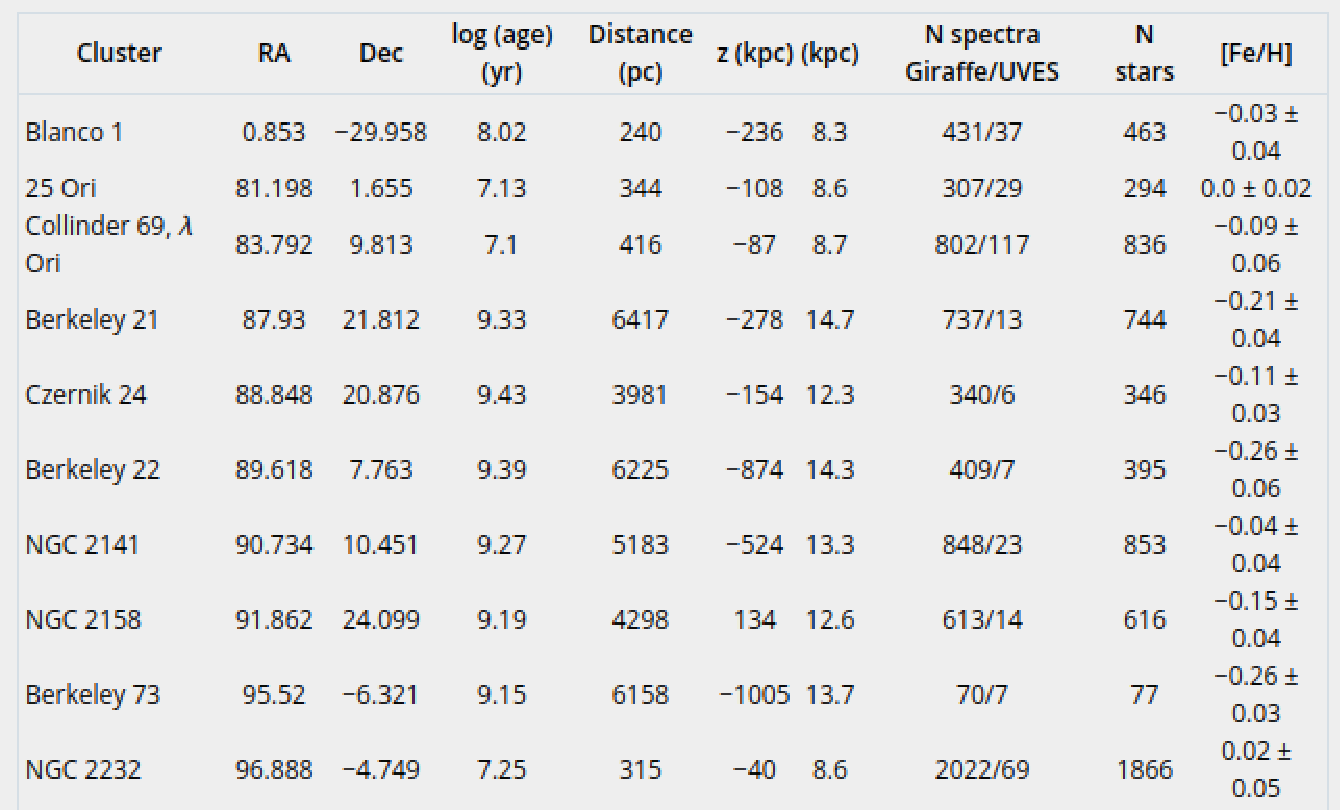
\includegraphics[width=0.7\textwidth]{img/tesis/open_cluster_sample.pdf}
	\caption{Tabla obtenida de \cite{Bragaglia2022}. Las columnas 1 a 7 listan la denominación del cúmulo, las coordenadas de ascensión recta y declinación, la edad estimada del cúmulo, la distancia (módulo de distancia convertido) en parsecs (pc) , la posición Z en coordenadas cartesianas galácticas, y la distancia desde el centro galáctico suponiendo que el Sol está a 8340 pc. Las columnas 8 y 9 enumeran el número de espectros y objetivos, mientras que la media de [Fe/H] y la desviación estándar se dan en la columna 10.}
	\label{fig:open_cluster_sample}
\end{figure}


\endinput
%--------------------------------------------------------------------
% FIN DEL CAPÍTULO. 
%--------------------------------------------------------------------